\documentclass{article}
\usepackage{amsmath}
\usepackage[style=authoryear]{biblatex}
\usepackage{graphicx}
\usepackage[]{hyperref}
\usepackage{tabularray}
\usepackage{siunitx}
\usepackage[noabbrev]{cleveref}
\addbibresource{bib/PhD.bib}
\begin{document}

\author{\and{Luke Thomas Smith} \and{Eun-Jung Holden} \and{Tom Horrocks} \and{Daniel Wedge} \and{Naveed Akhtar}}
\title{Super-Resolving Geophysical Surveys with Implicit Functions}
\date{\today}
\maketitle{}

\begin{abstract}
    Hi
\end{abstract}

\section{Introduction}
The analysis of potential field geophysical surveys relies on gridded sample data.
Sampling density and subsequent gridding processes impose limits on the observable detail in these data.
Recent work with both images and geophysical data has shown that these limits can be partially overcome using deep learning \parencite{moserHitchhikerGuideSuperResolution2023,smithMagneticGridResolution2022}.
However, the extent to which low-resolution geophysical data can be enhanced, the maximum useful upscaling factor, and characteristics of the resulting features remain to be fully explored.
These can be examined using the current generation of super-resolution networks, using arbitrary resolution, Multi-Layer Perceptron implicit functoin neural networks.

The first generation of super-resolution neural networks, starting with SRCNN \parencite{dongLearningDeepConvolutional2014}, were capable of upscaling at fixed factos with encouraging performance.
However, a separate trained model is required for each upscaling factor of interest, and performance beyond four time upscaling is modest.
Contemporary super-resolution can achieve arbitrary upscaling at larger factors using MLP implicit function super-resolution.
Implicit functions parameterise a function with a neural network analogue, which can be queried for information that fits the learnt function but was not represented by the training data.

One application of implicit neural networks is super-resolution (SR), the task of predicting interpolating values to resolve data in a higher resolution.
This task has previously been perfomed predominantly in the domain of Convolutional Neural Networks (CNN).
When compared to numerical methods such as bicubic filters, existing CNN based super-resolution methods for geophysical grids can predict infill pixels that add high frequency information which is repoted to be more accurate when compared to a ground trugh target \parencite{smithMagneticGridResolution2022}.
However, MLP based implicit networks can surpass CNNs for continuous domain super-resoltion with their explicit use of spatial coordinate features, such as pixel indices.
Be learning a signal as a function of its coordinates, arbitrary and continuous super-resolution is made possible bu predicting cell values at arbitrarily fine grid cell spacings.
While earlier CNN based SR methods can achieve upscaling at any trained scale factor, they require a bespoke model for inference at each different scale.
Using implicit functions, a single trained model is capable of high quality, arbitrary interpolation of the geophysical potential field, including at scales that were not seen during training.

\subsection{Resolution in geophysical surveys}
In exploration geophysics, the earth's naturally occurring magnetic or gravitational potential fields can be used to survey the petrophysical expression of the underlying geology.
Depending on the scale of investigation, surveys may be carried out from ground or airborne sensors, in a range of sampling regimes.
Detailed ground-based surveys can be sampled at point spacings of tens of metres while avoiding local obstacles, but at a regional scale, aircraft are used to provide rapid and uniform coverage regardless of access constraints.
These airborne surveys collect data at wider line spacing to minimise cost, typically between \SI{100}{\metre} and \SI{1000}{\metre}, but detailed surveys with line spacing closer than \SI{100}{\metre} are increasingly common.
Sampling along line is typically performed at \SI{10}{\hertz} or faster, which corresponds to several meters at a nominal flight speed of \SI{70}{\metre/\second} \parencite{goodwinAirborneMagneticRadiometric2023}.
Despite the use of precise navigation systems and skilled operators, these data are not collected in perfectly uniform lines at constant height, and the field samples also contain noise components.
Transforming these irregularly distributed line data to a uniformly spaced array is the challenge of regularisation.
Regularisation is performed by gridding, of which there are several distinct methods.
Minimum Curvature gridding \parencite{briggsMachineContouringUsing1974} is routinely applied in industry applications, as it gives good quality results in rapid time, with minimal manual intervention.
A comprehensive review of spatial interpolation methods is presented by \parencite{liReviewComparativeStudies2011}.
Each method of gridding has characteristic interpolation traits (which when undesired are termed artifacts), but irrespective of the gridding process, the detail resolvable in the output grid is a product of the final cell size.
Gridding at finer cell sizes preserves greater detail contained in the sampled data.

When the cell size covers a quantified distance, the maximum resolvable detail can be expressed as a wavelength.
This is the grids Nyquist wavelength, and is equal to twice the gridded cell size.
This is also known as the Nyquist frequency, the well-known limit at which sampled signals may be incorrectly resolved due to under sampling.
For example, a potential field that lacks significant wavelength components shorter than \SI{200}{\metre} will be adequately resolved by a grid with a cell size of \SI{100}{\metre}, without spurious features known as aliasing.

Extending this concept, arbitrarily shrinking the cell size will not resolve additional detail, without also predicting features with wavelengths shorter than those already present in the data.
These are limited by the sample spacing during acquisition.
As an additional constraint on the observable detail in sampled potential fields, the power of shorter wavelengths diminishes with increasing distances from the source.
Thus, potential fields grow smoother at larger source-sensor separation.

Considering all the factors that the limit the representation of short wavelength features in geophysical grids, accurately reconstructing or rediscovering any geologically significant features that have been lost during the survey and gridding process appears challenging.

\subsection{The benefit of higher resolution}
The nominal target resolution for different mapping scales depends on a survey's objectives, but in the absence of logistical constraints, higher resolution is preferred.
From visual observation, the benefits of higher resolution gridded geophysical data are obvious.
Details confined to short wavelengths such as near surface magnetic sources or small-scale structures are better localised and made more apparent in high resolution.
These features may provide important geological context, or better delineate structures manifested in the data.
In addition to human interpretation, machine processing of geophysical data is benefitted by using higher resolution data, with the typically negligible cost of increased computational load \parencite[e.g.][]{fitzgeraldArtificialIntelligenceTechniques2021}.

\subsection{Enhancing grid detail}
In order to resolve additional detail without additional sampling, it is required to predict the values of missing sample points.
Numerically, this can be done by interpolating functions, such as splines \parencite{keysCubicConvolutionInterpolation1981} or nearest neighbour methods.
These methods are limited in their performance by the quality of their neighbouring observed values, and their distance.
Deep learning methods also use their spatial neighbours, but do so in the context of trainable filters, and across larger extents of the input.
In this way, deep learning super-resolution upscaling models are supported by latent information retained from the training dataset, in addition to information contained within the input being upscaled.
For photographs and natural image rasters with large representative training corpuses available, such as ImageNet \parencite{dengImageNetLargescaleHierarchical2009} and DIV2K \parencite{agustssonNTIRE2017Challenge2017}, super-resolution methods have progressed to the point that high quality enhancement at four times scale in each axis is readily accessible to end-users \parencite[e.g.][]{wangRealESRGANTrainingRealWorld2021}.

Photographs and other rasters of interest to computer vision are typically created by capturing light from an image sensor or are explicitly mapped on a grid using a raster graphics program.
These data are encoded to regular arrays of pixel values, commonly as three-channel rasters representing the red, green, and blue intensities of each pixel.
In these rasters, each pixel is regularly distributed, and the resolution is isotropic and solely a factor of the pixel density of the sampling or constructed grid.
Contrastingly, geophysical grid rasters are created by point sample regularisation.
These point samples are irregularly spaced and often directionally dependent, especially in the case of airborne flight line sampling.
The resulting grid rasters may have isotropic cell size, but the frequency content in each axis is anisotropic, being a factor of the sample spacing and direction.
These grids also single channel, storing measurements of the geophysical property of interest.

A property of potential fields is that the power in high frequencies decreases with greater distance from the source.
At large source-sensor separations, higher frequencies are diminished below the noise floor to the point of unobservability, resulting in grids that show only broad scale features --- typically representing spatially extensive features deeper in the crust.
One method of restoring high frequency information to these grids is to calculate the potential as if it were sampled at a smaller source-sensor distance.
This is known as downward continuation \parencite{bullardDeterminationMassesNecessary1948}.
It is common for noise in the sampled grid product to be significantly worsened in the downward continued product, limiting the useful vertical extent of the method 6 times the cell size \parencite{dampneyEquivalentSourceTechnique1969,zuoDownwardContinuationTransformation2020}.
Once an independent signal has vanished below the noise floor, it is impossible to recover separately from noise components.
Downward continuation can be performed with field- or source-based methods \parencite{pilkingtonPotentialFieldContinuation2017}.

Recently, resolution enhancement with short wavelength prediction has been performed with deep learning super-resolution \parencite{smithMagneticGridResolution2022}.
While this method is capable of predicting short wavelengths and accurately super-resolving low-resolution magnetic grids, the data resolution was not limited by sample spacing, but rather a polynomial filter that supressed high frequencies.
Additionally, the trained network was limited to \num{4} times upscaling during inference.

\subsection{Convolutional neural networks for super-resolution}
Convolutional Neural Network (CNN) methods have long been well suited for computer vision tasks such as image classification and, more recently, super-resolution.
CNNs excel in deep learning tasks for raster data, due in part to the receptive field of the network.
The receptive field is formed from stacked layers of small convolutional kernels, typically with a size of 3x3 cells for modern CNNs.
These low-level kernels learn simple functions, which are convolved with deeper layers to learn increasingly complex filters across a larger image extent, widening the receptive field.
In an image, local features define important structures, which, as the network deepens, combine in the wider receptive field to define more global features.
Once trained, these filters are conditioned to transform low-resolution features into high-resolution features, using the neighbouring input values of the low-resolution grid in the context of filters learnt from the training data.

\begin{figure}[hbt]
    % 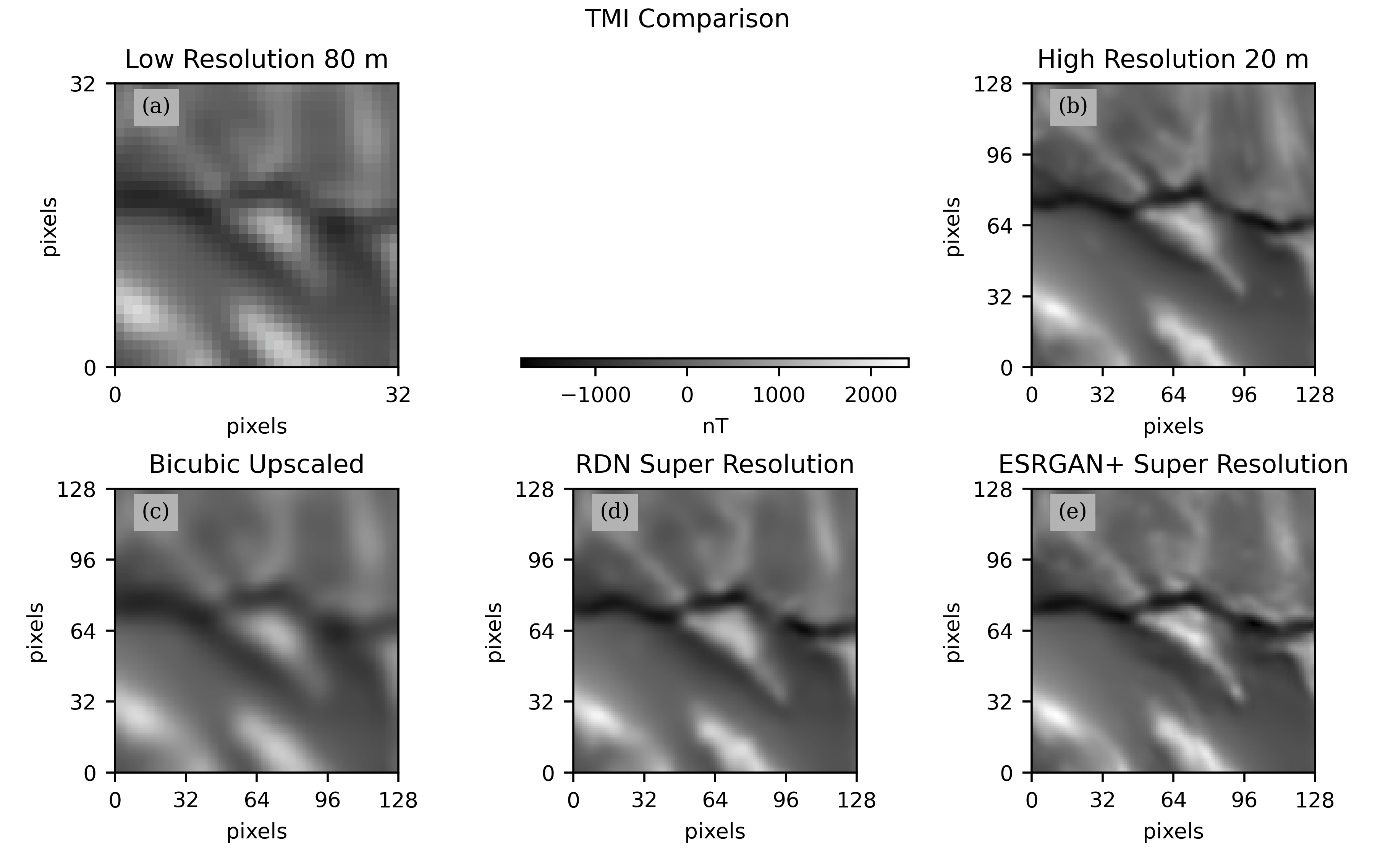
\includegraphics[width=\textwidth]{fig/p2/image1.png}
    \caption[An example CNN]{
        An example deep learning Convolutional Neural Network (specifically RDN (Zhang et al., 2018)), showing a variety of convolution operations (blue rectangles), activation functions (orange), and intermediate pathways (green, blue, or black arrows).
        }
    \label{fig:egcnn}
\end{figure}

The earliest application of deep learning super-resolution was demonstrated by \parencite{dongLearningDeepConvolutional2014,dongImageSuperresolutionUsing2016}, which uses convolutional layers for low-resolution patch extraction, mapping, and reconstruction of high-resolution images.
These layers are analogous to hand-crafted processes in contemporary example-based super-resolution methods, but are fully trainable with the deep learning approach.
Following the success of \cite{dongLearningDeepConvolutional2014}, many iterative improvements have been made to CNN based SR\@.
These include SRCNN \parencite{dongImageSuperresolutionUsing2016}, RDN \parencite{zhangResidualDenseNetwork2018}, ESRGAN \parencite{wangESRGANEnhancedSuperresolution2018}, and others \parencite{ledigPhotorealisticSingleImage2017,limEnhancedDeepResidual2017}.
While each of these works contributes unique features to CNN based super-resolution, they follow a common design.
This comprises a set of initial input feature extraction convolutions, a sequence of convolutional blocks with activations (neurons), some number and arrangement of intermediate residual learning pathways (skip connections), and an upsampling block for feature upscaling and convolving latent features back to image space e.g. \cref{fig:egcnn}.
Additionally, a majority of contemporary super-resolution networks investigate upscaling at a fixed scale, typically 4x.
While these networks can be trained for different factors using an appropriately scaled training dataset, they are constrained during inference to factor they are trained for.
Arbitrary scale super-resolution has been achieved using convolutional networks, notably Meta-SR \parencite{huMetaSRMagnificationarbitraryNetwork2019} and scale-arbitrary SR \parencite{wangLearningSingleNetwork2021}.
However, these methods perform poorly on novel data outside of their training scale distribution \parencite{chenLearningContinuousImage2021}. 

\subsection{Multi-layer Perceptron neural networks}
While Multi-layer Perceptron networks (MLP) have been used in science for decades, until recently networks partly or entirely comprising fully connected layers were not known for super-resolution.
\cite{tangDeepResidualNetworks2020} use stacked convolutional blocks for feature extraction, with a final fully connected layer for reconstructing a super-resolved image from the extracted features.
They suggest an MLP layer performs better for image reconstruction than a convolutional layer due to the wider receptive field of the MLP\@.
In an MLP, all neurons in each layer are connected to all neurons in the adjacent layer.
This contrasts with convolutional neural networks, where array elements are combined by the convolutional kernel as it feeds into deeper layers, which causes them to be sparsely connected.
A 1x1 convolutional kernel is occasionally considered analogous to an MLP\@.
Only in recent years have MLP based networks become a state-of-the-art alternative for super-resolution.

\begin{figure}[hbt]
    % 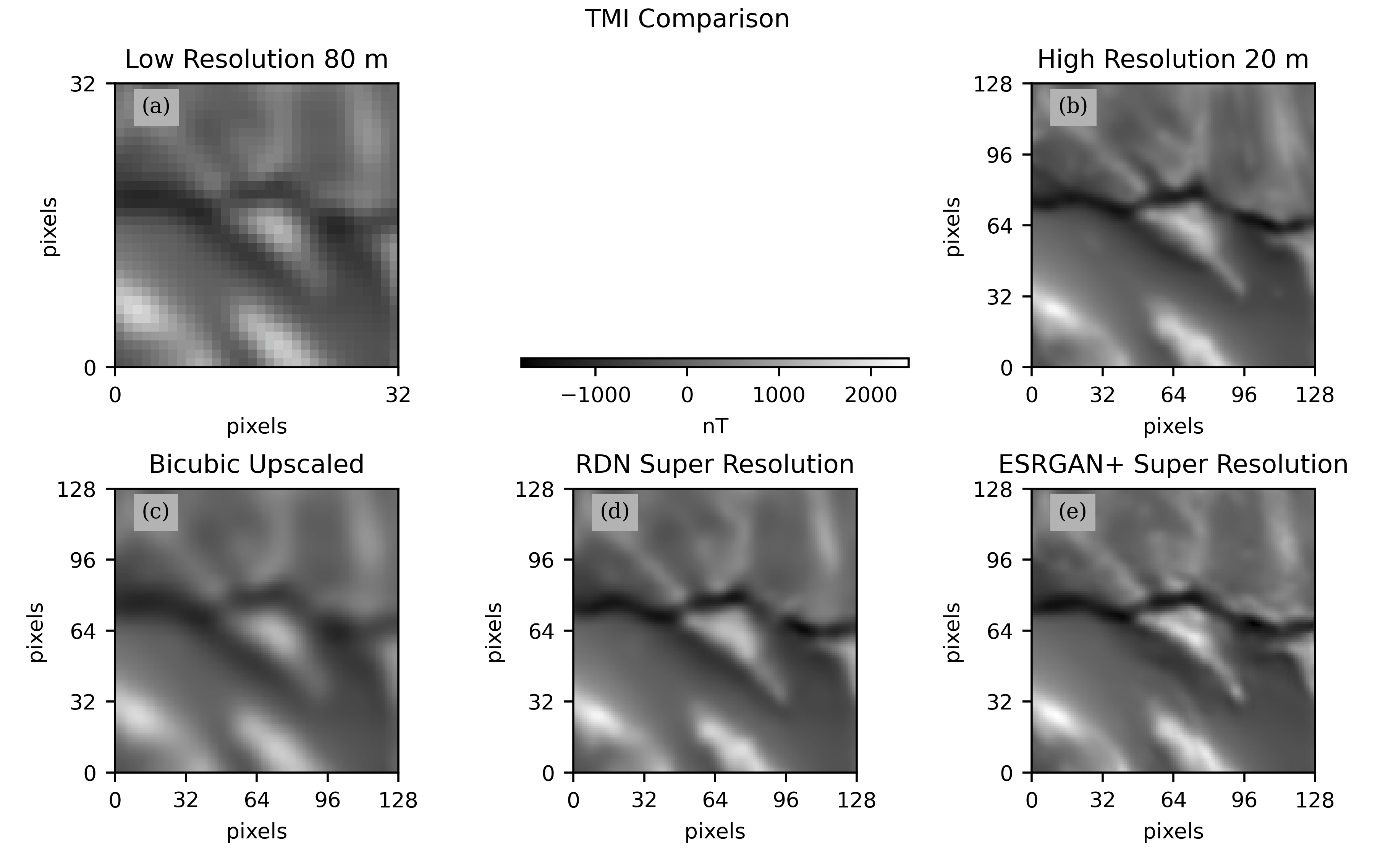
\includegraphics[width=\textwidth]{fig/p2/image1.png}
    \caption[An example deep learning Multi-layer Perceptron]{
        The encoder, $E_\Phi$, can be implemented as a feature extractor based on RDN prior its upsampling layer \cref{fig:egcnn} or SwinIR \parencite[per][]{leeLocalTextureEstimator2022}.
        $f_\theta$ is an MLP network used as the decoder for image reconstruction.
        A long-range skip connection with simple upscaling allows low-resolution information to bypass the network.
        }
    \label{fig:egmlp}
\end{figure}

\subsection{Implicit functions with multi-layer perceptron neural networks}
Implicit functions aim to learn a specific function parameterised entirely by the weights of a neural network.
In an image or geophysical grid context, the function maps grid coordinates to the value at those coordinates.
While extensively developed for point cloud and other 3D data \parencite[e.g.][]{jiangLocalImplicitGrid2020}, there have been numerous examples for super-resolution.
These include SIREN \parencite{sitzmann2019siren}, LIIF \parencite{chenLearningContinuousImage2021}, and LTE \parencite{leeLocalTextureEstimator2022}.
Notably in these networks, the learnt function has continuous domain, despite the discretised input.
Super-resolution can be achieved by sampling the learnt function at any arbitrary grid cell size smaller than the original input \parencite{chenLearningContinuousImage2021}.
While a stand-alone MLP such as SIREN is capable of parameterising a single function, when used in an autoencoder framework (such as with LIIF and LTE), an arbitrary input can be encoded using a CNN, upscaled, and reconstructed using fully connected layers \cref{fig:egmlp}.
This approach generalises MLP based super-resolution to any image or grid, even those not seen in the training set.


\subsection{Local Texture Encoder}
Examples of MLP based autoencoders for for learning continuous image representation super-resolution are LIIF \cite{chenLearningContinuousImage2021} and  LTE \cite{leeLocalTextureEstimator2022}.
While both are structured as autoencoders, with a CNN or transformer-based encoder followed by an MLP decoder, LTE is selected for its higher performance in the image super-resolution domain compared to LIIF\@.
The CNN encoder in these networks can use the feature extraction capacity of traditional SR CNNs such as EDSR \parencite{limEnhancedDeepResidual2017} or RDN \parencite{zhangResidualDenseNetwork2018}, without their upscaling blocks.
Lee and Jin find LTE achieves higher performance when using a SwinIR transformer based encoder.
In the original implementation of these CNN SR networks, the extracted image features are upscaled and returned to “image-space” by convolutional layers to reshape to image dimensions.
In LTE and LIIF, the extracted features become latent features with identical dimension as the original input image and are further processed by the network, before reconstruction to image space by an MLP\@.
Additionally, of interest to geophysics, a significant proportion of the LTE super-resolution network is trained on features in the Fourier domain.
The encoder extracts image features, but these are immediately transformed to the frequency domain by fully trainable convolution layers, which output amplitude and frequency features.
Phase features are also extracted from the image by a fully connected network, and is used during image reconstruction.
Nearest neighbour upsampling is performed in the frequency domain to achieve the required output scale.
A long-range skip connection passes low-frequency image content to the output of the network, in order to emphasise the learning of high-frequency content within the network.

\section{Material and Methods}
\subsection{Synthetic dataset}
%TODO

\section{Declaration of Competing Interest}
The authors declare the following financial interests / personal relationships which may be considered as potential competing interests: This work was supported by a Rio Tinto Iron Ore PhD scholarship.

\printbibliography{}


\end{document}